\chapter{Methodology}
\label{ch:methodology}
The methodology used to develop our hybrid music recommender consists of four main stages. First, the collection of real world user-item data corresponding to the play counts of specific songs and the fetching of audio clips of the unique identified songs in the dataset. Secondly, the implementation of the CDNN to represent the audio clips in terms of music genre probabilities as n-dimensional vectors. Next, permutation EDA and a continuous EDA are investigated to model user profiles based on the rated songs above a threshold. Finally, the process of top-N recommendation for the baseline and the hybrid recommender is described.

Every stage of our hybrid recommender is entirely developed in Python 2.7\footnote{https://www.python.org/download/releases/2.7/}, although, they are implemented in different platforms, e.g., OS X (v10.10.4) for the most part of the implementation, Ubuntu (14.04 LTS installed on VirtualBox 5.0.0) for intermediate time-frequency representation and CentOS (Linux release 7.1.1503) for the data preprocessing and CDNN implementation.

\section{Data collection}
The Million Song Dataset \parencite{Bertin-Mahieux2011} is a collection of audio features and metadata for a million contemporary popular music tracks which provides ground truth for evaluation research in MIR. This collection is also complemented by the Taste Profie subset which provides 48,373,586 triplets, each of them consist of anonymised user ID, Echo Nest song ID and play count. We choose this dataset because it is publicly available data and it contains enough data for user modelling and recommender evaluation.

\subsection{Taste Profile subset cleaning}
Due to potential mismatches\footnote{http://labrosa.ee.columbia.edu/millionsong/blog/12-2-12-fixing-matching-errors} between song ID and  track ID on the Echo Nest database, it is required to filter out the wrong matches in the Taste Profile subset. The cleaning process is illustrated in Figure~\ref{fig:taste_profile} 
\begin{figure}[ht!]
	\centering
	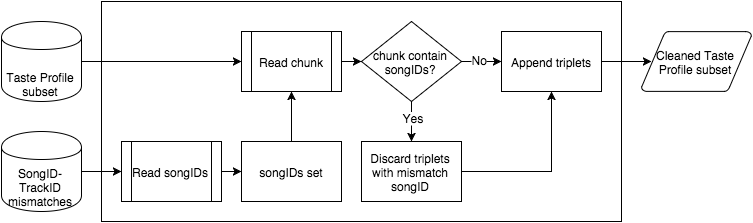
\includegraphics[width=0.9\textwidth]{chapter3/taste_profile.png}
	\caption{Diagram of the cleaning process of the Taste Profile subset}
	\label{fig:taste_profile}
\end{figure}
%Please see figure ~\ref{fig:JobInformationDialog} 

A script is implemented to discard the triplets that contain the song identifiers from the mismatches text file. First, we load the file to read each line of it to obtain song identifier. The identifiers are stored as elements of a set object to construct a collection of unique elements. Next, due to the size of the Taste Profile subset (about 3 GB, uncompressed), we load the dataset by chunks of 20,000 triplets in a \textit{pandas}\footnote{http://pandas.pydata.org/} dataframe to clean each chunk by discarding the triplets that contains the song identifiers in the set object of the previous step. The cleaning process takes around 2.47 minutes and we obtain 45,795,100 triplets. 

In addition to the cleaning process, we reduce significantly the size of the dataset for experimental purposes. We only consider users with more than 1,000 played songs and select the identifiers of 1,500 most played songs. This additional process takes around 3.23 minutes and we obtain 65,327 triplets. The triplets are stored in a cPickle\footnote{https://docs.python.org/2/library/pickle.html\#module-cPickle} data stream (2.8 MB).

%count resulting number of triplets
%At this stage, similarities between users is calculated to form a neighbourhood and predict user rating based on combination of the ratings of selected users in the neighbourhood.

\subsection{Fetching audio data}
First, for each element of the list of 1,500 songs identifiers obtained in the previous step is used to retrieve the associated Echo Nest track ID through a script using the \emph{get\_tracks} method from the \textit{Pyechonest}\footnote{http://echonest.github.io/pyechonest/} package which allow us to acquire track ID and preview URL for each song ID through Echo Nest API. The reason behind this is 7digital API uses Echo Nest track ID instead of song ID to retrieve any data from its catalogue. If the track information of a song is not available, the script skips to retrieve the Echo Nest information of the next song ID. At this point, it is useful to check if the provided 7digital API keys, a preview URL, and the country parameter, e.g., 'GB' to access to UK catalogue, work in the \textit{OAuth 1.0 Signature Reference Implementation}\footnote{http://7digital.github.io/oauth-reference-page/}.

Next, for each preview URL, we can create a GET request using \textit{python-oauth2}\footnote{https://github.com/jasonrubenstein/python\_oauth2} package, because it allows us to assign the nonce, the timestamp, the signature method and the country parameters. The request is converted to a URL to be opened with \textit{urlopen} function from the \textit{urllib2}\footnote{https://docs.python.org/2/library/urllib2.html} module, to download a MP3 file (44.1 kHz, 128 kbps, stereo) of 30 to 60 seconds of duration in a song repository.

Considering the Echo Nest API and 7digital API limited number of requests (see Section~\ref{sec:musicservices}), the process of fetching data from 1,500 song IDs takes at least 8 hours, resulting in a total of 640 MP3 files.

Additionally, the script accumulates the Echo Nest song identifier, track ID, artist name, song title and the 7digital preview audio URL for each downloaded track in a text file only if the audio clip is available for download. The generated text file is used for the preprocessing of the cleaned taste profile dataset in subsection~\ref{subsec:rating}. The flowchart of the script is shown in Figure~\ref{fig:fetchaudio}
\begin{figure}[ht!]
	\centering
	\includegraphics[width=0.9\textwidth]{chapter3/fetch_audio.png}
	\caption{Flowchart of the fetching audio process}
	\label{fig:fetchaudio}
\end{figure}

%include number of tracks available

%Classifier creates a model for each user based on the acoustic features of the tracks that user has liked.
\subsection{Intermediate time-frequency representation for audio signals}
\label{subsec:spectrogram}
Intermediate audio representation instead of waveform (time-domain) representation is required to feed a CDNN according to \textcite{NIPS2013_5004}. The flowchart to obtain the time-frequency representation from raw audio content of the song repository assembled in the previous section is shown in Figure~\ref{fig:timefrequency}.
\begin{figure}[ht!]
	\centering
	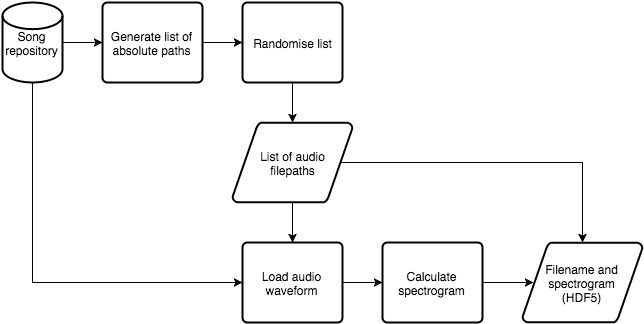
\includegraphics[width=0.7\textwidth]{chapter3/time_frequency.png}
	\caption{Flowchart for time-frequency representation process}
	\label{fig:timefrequency}
\end{figure}

First, a list of absolute paths corresponding to the songs in the repository is generated. The sequence of paths in the list is modified by random shuffling. This new sequence of absolute paths is saved in a text file.

Second, for every path in the text file of randomised absolute paths, a fragment equivalent to 3 seconds of the associated audio clip is loaded at a sampling rate of 22,050 Hz and converted to mono channel. For every fragment, a mel-scaled power spectrogram with 128 bands is computed from windows of 1,024 samples with a hop size of 512 samples, resulting in a spectrogram of 130 frames with 128 components. Hence, the spectrogram is converted to logarithmic scale in dB using peak power as reference. The functions \textit{load}, \textit{feature.melspectrogram} and \textit{logamplitude}, correspondingly to load an audio clip, spectrogram computation and logarithmic conversion, from the LibROSA\footnote{https://bmcfee.github.io/librosa/index.html} package are used.

To handle audio with LibROSA functions, it is recommended to use the Samplerate\footnote{https://pypi.python.org/pypi/scikits.samplerate/} package for efficient resampling. In our project, we considered to use the SoX\footnote{http://sox.sourceforge.net/} cross-platform without success due to operating system restrictions. Alternatively, we use the FFmpeg\footnote{https://www.ffmpeg.org/} cross-platform and \textit{libmp3lame0}\footnote{http://packages.ubuntu.com/precise/libmp3lame0} packages for efficient resampling.

Finally, we store the absolute path and the log-mel-spectrogram values of the 640 songs in a HDF5\footnote{https://www.hdfgroup.org/HDF5/} data file.

In the particular case for the time-frequency representation of each audio clip in the GTZAN dataset, we generate a list of the genre associated to each audio fragment that represent the target values (ground truth). This procedure for the GTZAN dataset is repeated for 9 times, considering the rest of 3-seconds fragments in each audio clip of the dataset for training, validation and testing of the CDNN (see Section~\ref{subsec:genre})

The time elapsed to obtain the time-frequency representation of the clips in the GTZAN dataset with the procedure described above is about 55 seconds, generating a HDF5 file (66.9 MB). Because of the number of MP3 files in the song repository is less than the number of files of the GTZAN dataset, the process is faster and the size of the HDF5 file is smaller (42.8 MB).

\section{Data preprocessing}
In order to obtain suitable representations for users' interest in the taste profile dataset and for songs' spectrograms, it is necessary an additional process of the data.
\subsection{Rating from implicit user feedback}
\label{subsec:rating}
First, the text file of the downloaded MP3 metadata (see subsection~\ref{subsec:spectrogram}) is used to retain the triplets, from the cleaned taste profile subset, that contain the song IDs of the available audio clips. A reduced taste profile dataset with 4,685 triplets is obtained, corresponding to information of 53 users.

The reduced taste profile dataset represent the user listening habits as implicit feedback, i.e., play counts of songs, it is necessary to normalise the listening habits as explicit feedback, i.e., range of values $[1\ldots5]$ that indicate how much a user likes a song. Normalisation of play counts is computed with the complementary cumulative distribution of play counts of a user, following the procedure given by \textcite{1242}. Songs in the top 80 - 100\% of the distribution get a rating of 5, songs in the 60 - 80\% range get a 4, songs in the 40 - 60\% range get a 3, songs in the 20 - 40\% get a 2 and songs in the 0 - 20\% range get a rating of 1. An exception for this allocation of ratings comes out when the coefficient of variation, given by Equation~\eqref{eq:cv}:
\begin{equation}
CV=\frac{\sigma}{\mu}
\label{eq:cv}
\end{equation}
where, $\sigma$ is the standard deviation and $\mu$ is the mean of the play counts of a user, is less or equal than $0.5$. In that case, every song gets a rating of 3.

\subsection{Standardise time-frequency representation}
\label{subsec:normalised}
The logarithmic mel-scaled power spectrograms obtained in subsection~\ref{subsec:spectrogram} are normalised to have zero mean and unit variance in each frequency band, using the \textit{fit} and \textit{transform} methods of the \textit{StandardScaler} class from the Scikit-learn~\parencite{scikit-learn} package, as a common requirement of several machine learning classifiers.

Additionally, the GTZAN normalised spectrograms dataset is split in 3 subsets: 500 spectrograms for training, 250 spectrograms for validation and 250 spectrograms for testing. Each spectrogram is saved as a tuple \textit{(spectrogram, tag)} in a cPickle file, where tag is the number of the music genre: 0 for blues, 1 for classical, 2 for country, 3 for disco, 4 for hiphop, 5 for jazz, 6 for metal, 7 for pop, 8 for reggae and 9 for rock.

\section{Algorithms}
\label{sec:algorithms}
The hybrid music recommender approach in this project can be considered as implementation of feature augmentation method and a meta-level method presented in subsection~\ref{subsec:hybridrecommender}. First, user profiles are generated using the rating matrix and the song vector representation. Next, the model generated is the input of a CB recommender to produce \emph{top-N} song recommendations. The general model of our hybrid recommender is shown in Figure~\ref{fig:generalhybrid}
\begin{figure}[ht!]
	\centering
	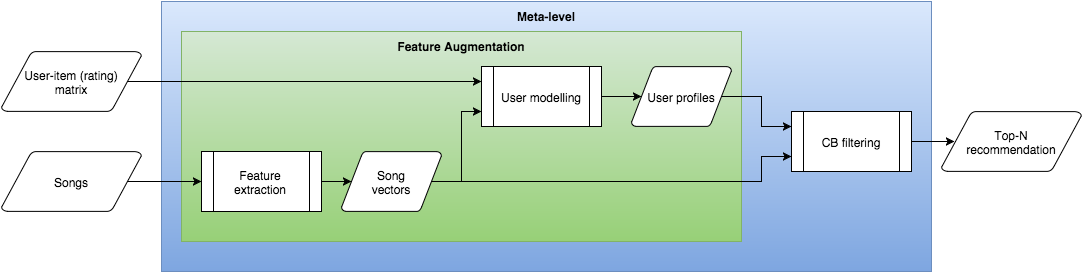
\includegraphics[width=\textwidth]{chapter3/General_model_hybrid_recommender.png}
	\caption{Diagram of the hybrid music recommender}
	\label{fig:generalhybrid}
\end{figure}

\subsection{Probability of music genre representation}
\label{subsec:genre}
To represent an audio file in a 10-dimensional vector, whose dimensions correspond to the 10 music genres specified in the GTZAN dataset, a CDNN is implemented using Theano library. For intensive computation processes, such as convolution, the implementation on equipment with Graphical Processing Unit (GPU) acceleration is recommended. In this project, a CentOS (Linux release 7.1.1503) server with a Tesla K40c\footnote{http://www.nvidia.com/object/tesla-servers.html} GPU is exploited.

The scripts for logistic regression, multilayer perceptron and deep convolutional network designed for character recognition of MNIST\footnote{http://www.iro.umontreal.ca/~lisa/deep/data/mnist/mnist.pkl.gz} dataset, available on~\textcite{1_deeplearning.net_2015} is adapted to our purpose of music genre classification. ReLU and dropout functions are defined in the deep convolutional network script.

%Deep belief network is a probabilistic model that has one observed layer and several hidden layers.
\subsubsection{CDNN architecture}
\begin{figure}[ht!]
	\centering
	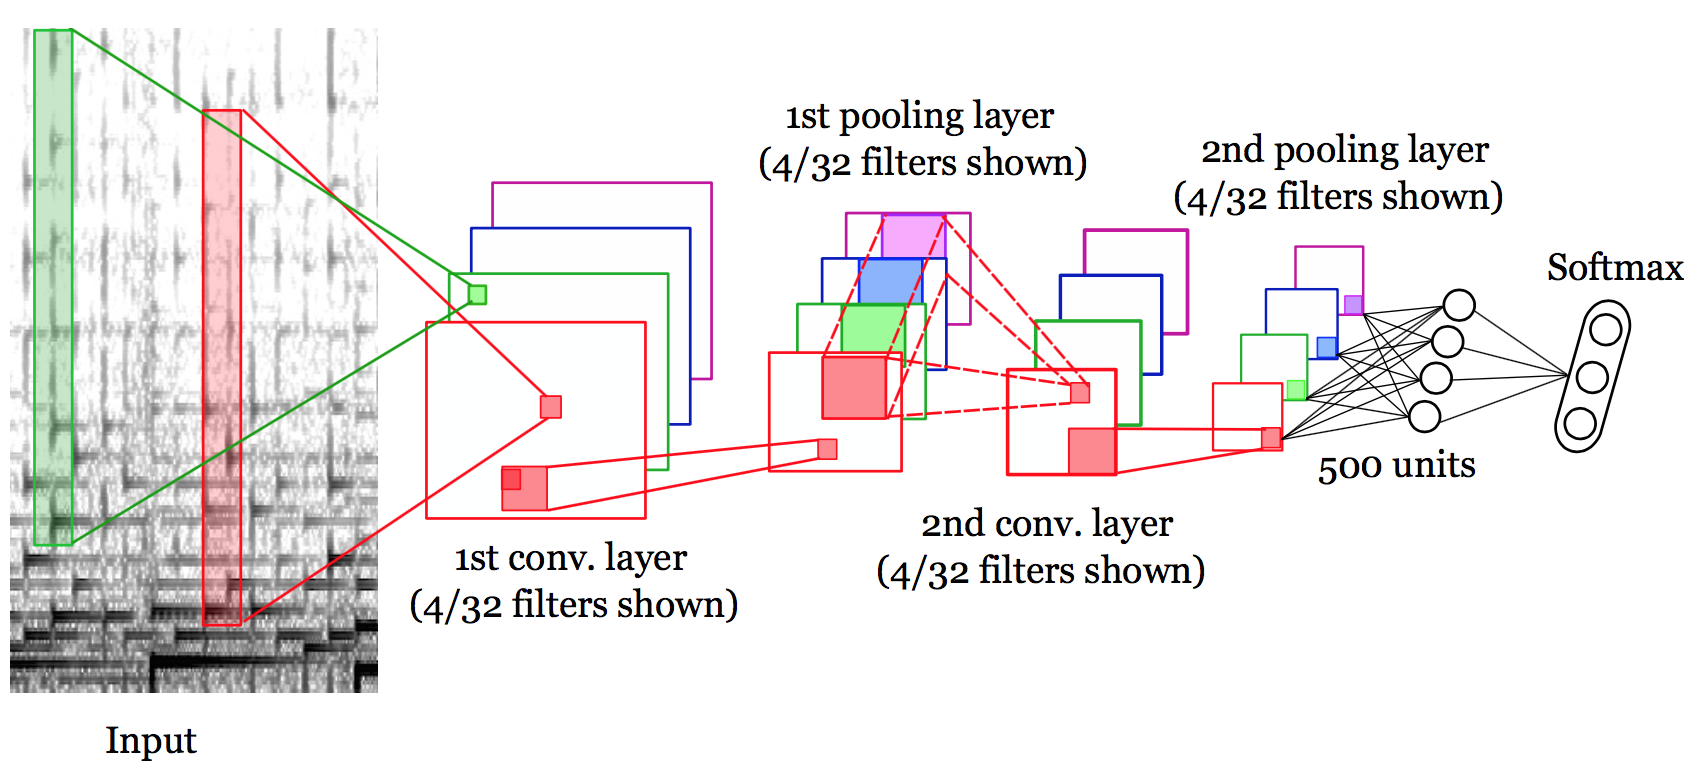
\includegraphics[width=\textwidth]{chapter3/CDNN.png}
	\caption{Diagram of CDNN for music genre classification~\parencite{kereliuk15}}
	\label{fig:cdnn}
\end{figure}
A similar architecture of a CDNN for music genre classification~\parencite{kereliuk15} is recreated in our project. A batch size of 20 and a dropout rate of 0.20 for the convolutional layer units are considered.

Initially, the reshape of the 2-dimension normalised spectrograms (130 frames$\times$128 frequency bands) obtained in subsection~\ref{subsec:normalised} to a 4-dimension tensor, compatible with the input of the first convolutional layer (batch size$\times$1$\times$130$\times$128), is required.

The first convolutional layer consists of 32 filters, each one with a size of 8 frames, with a max-pooling downsampling of 4, to reduce the size of the spectrogram along the time axis. The size of the resulting spectrogram is 30$\times$128 and the output of this first convolutional layer is a 4-dimension tensor with a size of 20$\times$32$\times$30$\times$128.

The second convolutional layer consists of 32 filters, each one with a size of 8 frames, with a max-pooling downsampling of 4, to reduce the size of the spectrogram obtained in the first layer. The size of the new spectrogram is 5$\times$128 and the output of this second convolutional layer is a 4-dimension tensor with a size of 20$\times$32$\times$5$\times$128.

Following the convolution process, the reshape of the 4-dimensional tensor of the output of the second convolutional layer is required to feed the fully connected MLP. The MLP consists of 500 ReLUs.

Finally, the classification of music genre is accomplished with logistic regression layer of the 500 output values from the MLP. This output layer consists of 10 units with softmax activation function (see Equation~\eqref{eq:softmax}).

\subsubsection{Learning parameters}
The weights and biases of the units of the CDNN are the parameters
to be modelled by SGD to minimise a cost function. The cost function is the negative log likelihood of the prediction in the output layer given the target values, i.e., music genre ground truth.

The CDNN for training, validation and testing is run for 200 epochs, each epoch equivalent to 50 iterations. The number of iterations corresponds to the ratio between the number of spectrograms (1,000 for GTZAN dataset) and the batch size.

According to \textcite{bengio2012practical}, the patience value is the minimum number of training examples. In our project, the patience value is set at 1,000.

In our testing, after 9 trials in the CDNN, we obtain a best classification error of 38.8 \% using the spectrograms corresponding to the GTZAN dataset (see Table~\ref{table:genre}). The weights and biases for this best classification error are saved in a cPickle file to be applied as initial parameters of the CDNN for vector representation.

\subsubsection{Vector representation}
The script of CDNN is adapted to produce the vector representation of the spectrograms. This CDNN uses the weights and biases learnt in genre classification process as initial parameters.

A 10-dimension vector is produced by the softmax output layer. Each dimension corresponds to a music genre and each value represents the probability of a song to belong to a specific music genre, given the normalised spectrogram at the input layer.

\subsection{User profile modelling}
\label{subsec:profile}
To model user profiles from the triplets in the normalised taste profile dataset, we adapt the permutation EDA (see algorithm~\ref{alg:hybrideda} on page ~\pageref{alg:hybrideda}) and the continuous EDA (see algorithm~\ref{alg:umda} on page ~\pageref{alg:umda}). For both EDAs, we consider the following:
\begin{itemize}
	\item User representation $S_u=\{(t_1, r_{u,1}),\ldots,(t_i, r_{u,i})\vert r_{u,i}>\bar r_{u}\}$.
	\item Rating threshold $\bar r_{u}\}=2$, assuming that a user does not like songs with ratings of 1 and 2 out of 5.
	\item The stopping criteria is the maximum number of generations limited to 250.
\end{itemize}


\subsubsection{Modelling with Permutation EDA}
In the case of permutation EDA, the genre tags (0 for blues, 1 for classical, 2 for country, 3 for disco, 4 for hiphop, 5 for jazz, 6 for metal, 7 for pop, 8 for reggae and 9 for rock) are considered as the keywords $k_n$ in the set $D_u$ and the weights $w_{n,i}$ are 50 evenly spaced samples over the interval $[0.1, 0.9]$, thus, the size of the set $K_u$ is $N=500$ and the initial probability is $c_{n,i}=1/500$.

The population size is equal to $u=53$, that is the number of users in the normalised taste profile dataset. Instead of using the Monte Carlo method to generate the initial population of $profile_u$, 10 tuples $(k_n,w_{n,i})$ from $K_u$ are random sampled for each user. The number of top individuals $M$ is a half of the total of users. The process of sampling new individuals is preserved. The adapted permutation EDA for user modelling is illustrated in Algorithm~\ref{alg:permutationeda}:

\begin{algorithm}[ht!]
	\caption{Calculate $profile_u$ for users in taste profile}
	\begin{algorithmic} 
		\REQUIRE set $D_u$, weights $w_{n,i}$
		\REQUIRE population size $u$, MAXGEN
		\REQUIRE $M = Round(u/2)$
		%\ENSURE $y = x^n$
		%\STATE Random selection of keywords $k_n$ from $D_u$
		\STATE Assign a weight $w_{n,i}$ to each $k_n$ to build a set~$K_u$ of size~$N$
		\STATE Assign a probability $c_{n,i}=1/N$ to each $(k_n,w_{n,i})$
		\STATE Generate initial population of $profile_u$
		\WHILE{$generation <$ MAXGEN}
		\STATE Compute each $fitness(profile_u)$
		\STATE Rank individuals by their fitness value
		\STATE Select top $M < N$ individuals
		\STATE Update $c_{n,i}$ by counting the occurrences of $(k_n,w_{n,i})$ in the $M$ individuals profiles
		\STATE Generate $profile_u$ by random sampling according to updated $c_{n,i}$
		\STATE $generation\leftarrow generation+1$
		\ENDWHILE
		\RETURN $profile_u$
	\end{algorithmic}
	\label{alg:permutationeda}
\end{algorithm}

The time elapsed for modelling user profiles with the permutation EDA is approximately 7.82 seconds.

\subsubsection{Modelling with $UMDA_c^G$}
The $UMDA_c^G$ algorithm is adapted to select the top $M_{sel}$ individuals by using the fitness function (Equation~\eqref{eq:fitness} on page~\pageref{eq:fitness}) exploited by the permutation EDA. The population size is $M=53$ users, the selection parameter is $\tau=0.5$. $x_i$ represent the probability value of the music genre dimension, \emph{i}, in the $profile_u$ vector.

In each generation, \emph{t}, the mean value $\mu_{i,t}$ and the variance $\sigma_{i,t}^2$ is computed for every dimension, $i$, along the $M_{sel}$ individuals vectors. For each dimension, i.e., music genre, the normal distribution is calculated with its corresponding mean value and variance, to estimate the  individuals vectors of the next generation.
\begin{algorithm}[ht!]
	\caption{Framework for $UMDA_c^G$ to model users}
	\begin{algorithmic} 
		\REQUIRE population size $M$
		\REQUIRE selection parameter $\tau$
		\STATE Generate $M$ individuals at random
		\STATE $M_{sel}\leftarrow M\cdot\tau$
		\STATE $t \leftarrow 0$
		\WHILE{$t <$ MAXGEN}
		\STATE Compute each $fitness(profile_u)$
		\STATE Rank individuals by their fitness value
		\STATE Select top $M_{sel}$ individuals 
		\STATE $\mu_{i,t}\leftarrow\frac{1}{M_{sel}}\sum_{j=1}^{M_{sel}}x_i^j$
		\STATE $\sigma_{i,t}^2\leftarrow\frac{1}{M_{sel}-1}\sum_{j=1}^{M_{sel}}(x_i^j-\mu_{i,t})^2$ 
		\STATE $p_t({x_{i}}\vert \mu_{i,t},\sigma_{i,t}^2)\leftarrow\frac{1}{\sqrt{2\pi}\sigma_{i,t}}\exp(-\frac{1}{2}(\frac{x_i-\mu_{i,t}}{\sigma_{i,t}})^2)$
		\STATE Sample $M$ individuals from $p_t({x_{i}}\vert \mu_{i,t},\sigma_{i,t}^2)$
		\STATE $t\leftarrow t+1$
		\ENDWHILE
	\end{algorithmic}
	\label{alg:umda2}
\end{algorithm}
The time elapsed for modelling user profiles with the continuous EDA is approximately 4.20 seconds.
\subsection{Top-N songs recommendation}
The final stage of the recommender systems implemented is to generate a list of song recommendations according to the similarity values computed with Equation~\eqref{eq:wpearson} (see page~\pageref{eq:wpearson}).
\subsubsection{Top-N recommendations in CB baseline}
The list of recommendations in a CB recommender is given by the similarities between the items that a user has already rated and the new items. It is assumed the user has not seen before the new items.

First, the similarity matrix between every item in the training set is computed. Only the $k=30$ most similar items are kept for each item. Next, for each song that a user rated above the threshold (rating $>$ 2), the $k$ neighbours are retrieved as a list of candidate items. The list is normalised to have a maximum value of 1. The lists of candidates are appended. For the repeated candidates, the similarity values are summed up. The $N$ candidates with higher similarity values are recommended to a user.

\subsubsection{Top-N recommendations in hybrid music recommender}
In our hybrid music model (see Figure~\ref{fig:generalhybrid} on page~\pageref{fig:generalhybrid}), the content based filtering computes the similarity between a user interest profile and a each song vector in the test set. The songs are ranked in descending order and the first $N$ songs of this ranking are recommended.

In our project, we experiment with different values for N, obtaining the best results with the hybrid music recommender based on permutation EDA for all the experiments. Refer to Section~\ref{sec:recresults} for detailed results of evaluation.

\section{Summary}
In this chapter, we presented the collection and preprocessing of the taste profile subset to model the user profiles with EDAs. As well, we presented the procedure of time-frequency representation of the audio content to feed a CDNN in order to obtain a 10-dimension vector representation corresponding to the probability of a song to belong to a music genre. Also, we presented the adapted architecture of the CDNN and the EDAs for hybrid recommendation. In the following chapter, we introduce the evaluation method and experiments to evaluate our hybrid recommender approach.